\section{Overapproximation of Synchronous Traces} \label{sec:approach}
In this section, given a distributed signal $(S,{\hb})$, we describe an overapproximation $\tr^+(S,{\hb})$ of its set $\tr(S,{\hb})$ of synchronous traces.
First, we present the notion of \emph{canonical segmentation}, a systematic way of partitioning the temporal domain of a given distributed signal to keep track of the partial asynchrony.
Second, we introduce the notion of \emph{value expressions}, sets of finite words representing how a signal behaves in a time interval.
Finally, we define $\tr^+$ based on these notions, and show that it soundly approximates $\tr$.

\begin{remark}
	We assume Boolean signals in this section for convenience (all results hold for non-Boolean 
	signals).
	%
	The definitions and results presented here extend to real-valued signals because finite-length piecewise-constant signals will only use a finite number of values.
\end{remark}

\subsubsection{Canonical Segmentation}
Consider a Boolean signal $x$ with a rising edge at time $t > \varepsilon$.
Due to clock skew, this edge occurs in the range $(t - \varepsilon, t + \varepsilon)$ from the monitor's point of view.
This range is called an \emph{uncertainty region} because in $(t - \varepsilon, t + \varepsilon)$ the monitor cannot tell the value of $x$ precisely, but only that it changes from 0 to 1.
Formally, given an edge $(t, x(t))$, we define $\theta_{\text{lo}}(x,t) = \max(0, t - \varepsilon)$ and $\theta_{\text{hi}}(x,t) = \min(d, t + \varepsilon)$ as the end points of the edge's uncertainty region.

Given a temporal domain $I = [0,d) \subset \R_{\geq 0}$, a \emph{segmentation} of $I$ is a partition of $I$ into finitely many intervals $I_1, \ldots, I_k$, called \emph{segments}, of the form $I_j = [t_j, t_{j+1})$ such that $t_j < t_{j+1}$ for all $1 \leq j \leq k$.
By extension, a segmentation of a collection of signals with the same temporal domain $I$ is a segmentation of $I$.

%Let $x : [0,d) \to \R$ be a signal and $(t, x(t))$ be an edge of $x$. %$E_x = \{(t_1, x(t_1)), \ldots, (t_m, x(t_m))\}$ be the set of edges of $x$, given in an increasing order of local clock values.
%We define $\theta_{\text{lo}}(x,t) = \max(0, t - \varepsilon)$ and $\theta_{\text{hi}}(x,t) = t + \varepsilon$.
%%\begin{align*}
%%	%	\theta_{\text{lo}}(x,t_i) &= \max\{0, \max_{j \in \{1, i\}} t_j - \varepsilon - (j-i)\delta\} \text{, and} \\
%%	\theta_{\text{lo}}(x,t_i) &= \max_{1 \leq j \leq i} t_j - \varepsilon + (i-j)\delta \text{, and} \\
%%	\theta_{\text{hi}}(x,t_i) &= \min_{i \leq j \leq m} t_j + \varepsilon - (j-i)\delta.
%%\end{align*}
%Intuitively, $\theta_{\text{lo}}$ and $\theta_{\text{hi}}$ give us the lower and upper bounds on the value of the monitor's clock for a given edge, i.e., the end points of the uncertainty region of the given edge.
%We use these to describe a canonical segmentation of a distributed signal.

Let $(S,{\hb})$ be a distributed signal of $n$ signals.
The \emph{canonical segmentation} $G_S$ of $(S,{\hb})$ is the segmentation of $S$ where the end points of the segments coincide with the end points of its temporal domain and uncertainty regions.
Formally, we define $G_S$ as follows.
For each signal $x_i$, where $1 \leq i \leq n$, let $F_i$ be the set of end points of its 
uncertainty regions.
%Let $d' = \max(d, \max (\bigcup_{i = 1}^{n} F_i))$, which corresponds to the duration of the distributed signal with respect to the monitor's clock.
%
Let $F = \{0, d\} \cup \bigcup_{i = 1}^{n} F_i$ and let $(s_j)_{1 
\leq j \leq |F|}$ be a nondecreasing sequence of clock values corresponding to the elements of $F$.
Then, the canonical segmentation of $(S,{\hb})$ is $G_S = \{I_1, \ldots, I_{|F| - 1}\}$ where $I_j = [s_j, s_{j+1})$ for all $1 \leq j < |F|$.

\begin{example} \label{ex:canonseg}
	Let $(S, {\hb})$ be a distributed Boolean signal with $S = (x_1, x_2)$ and $\varepsilon = 2$ over 
	the temporal domain $[0,8)$ as given in \cref{fig:canonseg}.
	Both signals are initially 0.
	The signal $x_1$ has a rising edge at time 2 and a falling edge at time 5, while $x_2$ has a rising edge at time 3 and a falling edge at time 6.
	The uncertainty regions of $x_1$ are $(0,4)$ and $(3,7)$, while those of $x_2$ are $(1,5)$ and $(4,8)$.
	Then, we have $F = \{0, 8\} \cup \{0, 1, 3, 4, 5, 7, 8\}$, and thus the canonical segmentation is $G_S = \{ [0,1), [1,3), [3,4), [4,5), [5,7), [7,8) \}$.
\end{example}

\begin{figure} 
	\centering
	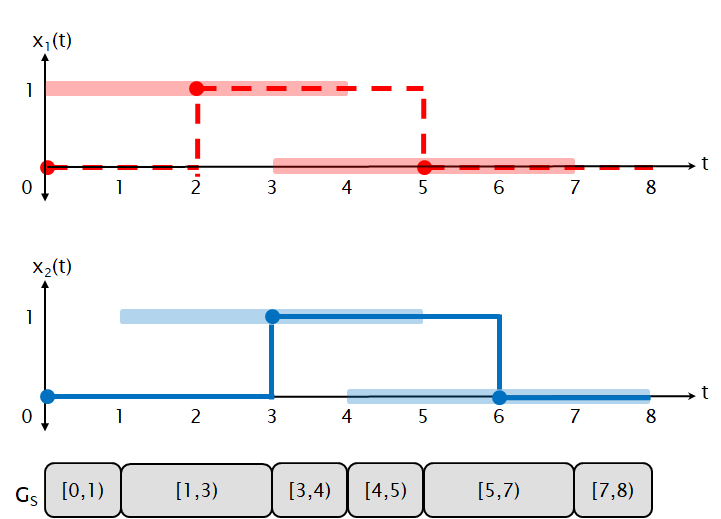
\includegraphics[scale=0.5]{canonseg.png}
	\caption{The signals $x_1$ (top, red, dashed) and $x_2$ (bottom, blue, solid) from \cref{ex:canonseg}. The edges are marked with solid balls and their uncertainty regions are given as semi-transparent boxes around the edges. The resulting canonical segmentation $G_S$ is shown below the graphical representation of the signals.}
	\label{fig:canonseg}
\end{figure}


\subsubsection{Value Expressions}
Consider a boolean signal $x$ with a rising edge with an uncertainty region of $(t_1, t_2)$.
As discussed above, the monitor only knows that the value of $x$ changes from 0 to 1 in this interval.
We represent this knowledge as a finite word $v = 01$ over the alphabet $\Sigma = \{0,1\}$.
This representation is called a \emph{value expression} and it encodes the uncertain behavior of an observed signal relative to the monitor.
Formally, a value expression is an element of $\Sigma^*$ where $\Sigma$ is the finite alphabet of values the signal takes.
Given a signal $x$ and an edge $(t, x(t))$, the value expression corresponding to the uncertainty region $(\theta_{\text{lo}}(x,t), \theta_{\text{hi}}(x,t))$ is given by $v_{x,t} = v_- \cdot v_+$ where $v_- = \lim_{s \to t^-} x(s)$ and $v_+ = \lim_{s \to t^+} x(s)$.
When drop the concatenation symbol $\cdot$ when the letters are clear from the context.
Let us remark that this definition is general because finite-length piecewise-constant real-valued signals will only have a finite number of values, making $\Sigma$ finite.

Notice that (i) uncertainty regions may overlap, and (ii) the canonical segmentation may split an uncertainty region into multiple segments.
Consider a signal $x$ with a rising edge in $(1,5)$ and a falling edge in $(4,8)$.
The corresponding value expressions are respectively $v_1 = 01$ and $v_2 = 10$.
Notice that the behavior of $x$ in the interval $[1,4)$ can be expressed as $\pfx(v_1)$, encoding whether the rising edge has happened yet or not.
Similarly, the behavior in $[4,5)$ is given by $\sfx(v_1) \cdot \pfx(v_2)$, which captures whether the edges occur in this interval (thanks to prefixing and suffixing) and the fact that the rising edge happens before the falling edge (thanks to concatenation).

Formally, given a distributed signal $(S,{\hb})$, we define a function $\gamma : S \times G_S \to 2^{\Sigma^*}$ that maps each signal and segment of the canonical segmentation to a set of value expressions, capturing the signal's potential behaviors in the given segment.
Let $x$ be a signal in $S$, and let $R_1, \ldots, R_m$ be its uncertainty regions where $R_i = (t_i, t_i')$ and the corresponding value expression is $v_i$ for all $1 \leq i \leq m$.
Now, let $I \in G_S$ be a segment with $I = [s, s')$ and for each $1 \leq i \leq m$ define the set $V_i$ of value expressions capturing how $I$ relates with $R_i$ as follows:
%
\small
\begin{equation} \label{eq:valexprset}
	V_i = 
	\begin{cases}
		\{v_i\} & \text{if } t_i = s \land s' = t_i' \\
		\pfx(v_i) & \text{if } t_i = s \land s' < t_i' \\
		\sfx(v_i) & \text{if } t_i > s \land s' = t_i' \\
		\infx(v_i) & \text{if } t_i > s \land s' < t_i' \\
		\{\epsilon\} & \text{otherwise}
	\end{cases}
\end{equation}
\normalsize
The last case happens only when $I \cap R_i$ is 
empty.
We finally define $\gamma$ as follows:
\[ \gamma(x,I) = \destutter(V_1 \cdot V_2 \cdot \ldots \cdot V_m) \setminus \{\epsilon\} \]
Observe that $\gamma(x,I)$ contains all the potential behaviors of $x$ in segment $I$ by construction.
However, it is potentially overapproximate.
This is mainly because the sets $V_1, \ldots, V_m$ contain redundancy by definition and the concatenation does not guarantee that an edge is considered exactly once.
%We demonstrate an example in \cref{fig:valexpr}.

\begin{example} \label{ex:valexpr}
	Recall the distributed signal $(S, {\hb})$ in \cref{ex:canonseg} and \cref{fig:canonseg}.
	In \cref{fig:valexpr}a, we show the value expressions corresponding to its uncertainty regions.
	For example, the falling edge of $x_1$ has an uncertainty region of $(3,7)$, represented by the value expression $10$.
	In \cref{fig:valexpr}b, we give the function $\gamma$ for $(S, {\hb})$.
	For example, $\gamma(x_1, [3,4)) = (\sfx(01) \cdot \pfx(10)) \setminus \{\epsilon\} = \{ 01, 010, 1, 10\}$, and 
	$\gamma(x_2, [0,1)) = \{0\}$.
\end{example}

\begin{figure} 
	\centering
	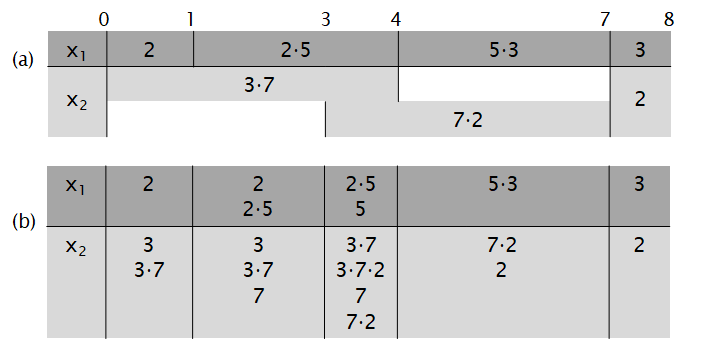
\includegraphics[scale=0.45]{valexpr.png}
	\caption{(a) The uncertainty regions of the distributed signal in \cref{ex:canonseg} and the corresponding value expressions. (b) The tabular representation of the function $\gamma$ for the given distributed signal.}
	\label{fig:valexpr}
\end{figure}

\subsubsection{Overapproximation of $\tr$.}
Consider a distributed signal $(S,{\hb})$ of $n$ signals, and let $G_S$ be its canonical segmentation.
We describe how the function $\gamma$ defines a set $\tr^+(S,{\hb})$ of synchronous traces that overapproximates the set $\tr(S,{\hb})$.
%
%Let $x : [0,d) \to \B$ be a signal.
%Consider the set $N_x$ of signals such that each $x' \in X$ is obtained from $x$ by shifting its edges within their uncertainty regions while preserving their relative order.
%Formally, we let $E = \{ (t_1, x(t_1)), \ldots, (t_m, x(t_m)) \}$ be the set of edges of $x$ with $t_i < t_{i+1}$ for all $1 \leq i < m$, let $R_1, \ldots, R_m$ be the corresponding uncertainty regions, and define $N_x$ as follows: 
%$$ N_x = \{x' : [0,d) \to \B \st x'(0) = x(0) \land \forall 1 \leq i \leq m : t_i' \in R_i \land x'(t_i') = x(t_i) \} $$ where $E' = \{ (t_1', x'(t_1')), \ldots, (t_m', x'(t_m')) \}$ is the set of edges of $x'$ with $t_i' < t_{i+1}'$ for all $1 \leq i < m$.
%For example, ...
%
%Now, 
%Let $x \in S$ and $x'$ be two signals with the same temporal domain, and let $I = [s, s')$ be a segment in $G_S$.
%Let $(t_1, x'(t_1)), \ldots, (t_\ell, x'(t_\ell))$ be the edges of $x'$ in segment $I$ with $t_i < t_{i+1}$ for all $1 \leq i < \ell$.
%The signals $x$ and $x'$ are \emph{consistent in $I$} iff $x(s) = x'(s)$ and the value expression $x'(s) \cdot x'(t_1) \cdot \ldots \cdot x'(t_\ell)$ belongs to $\gamma(x,I)$.
%Moreover, $x$ and $x'$ are \emph{consistent} iff they are consistent in $I$ for all $I \in G_S$.
%Now, let $S = (x_1, \ldots, x_n)$ and define the \emph{canonical overapproximation} of $(S,{\hb})$ as follows:
%$$ \tr^+(S,{\hb}) = \{ (x_1', \ldots, x_n') \st \text{$x_i$ and $x_i'$ are consistent for all $1 \leq i \leq n$}\} $$
%
Let $x \in S$ and $x'$ be two signals with the same temporal domain, and let $I = [s, s')$ be a segment in $G_S$.
Let $(t_1, x'(t_1)), \ldots, (t_\ell, x'(t_\ell))$ be the edges of $x'$ in segment $I$ with $t_i < t_{i+1}$ for all $1 \leq i < \ell$.
The signal $x'$ is \emph{$I$-consistent with $x$} iff the value expression $x'(s) \cdot x'(t_1) \cdot \ldots \cdot x'(t_\ell)$ belongs to $\gamma(x,I)$.
Moreover, $x'$ is \emph{consistent with $x$} iff it is $I$-consistent with $x$ for all $I \in G_S$.

Now, let $S = (x_1, \ldots, x_n)$ and define $\tr^+(S,{\hb})$ as follows:
\[ \tr^+(S,{\hb}) = \{ (x_1', \ldots, x_n') \st \text{$x_i'$ is consistent with $x_i$ for all $1 \leq i \leq n$}\} \]



\begin{example} \label{ex:overapx}
	Recall the distributed signal $(S, {\hb})$ in \cref{ex:canonseg} whose $\gamma$ function is given in \cref{fig:valexpr}b.
	Consider the synchronous trace $w \in \tr(S, {\hb})$ where the rising edges of both signals occur at time 3 and the falling edges at time 5.
	A signal such as $w$ would be included in $\tr^+(S,{\hb})$ since for each $i \in \{1,2\}$ the value expression 1 is contained in $\gamma(x_i, [3,4))$ and $\gamma(x_i, [4,5))$ while 0 is contained in the remaining sets $\gamma$ maps $x_i$ to.
	Now, consider a synchronous trace $(x_1', x_2')$ where both signals are initially 0, have rising edges at time 2 and 3.5, and falling edges at time 3 and 5.
	Evidently, this trace does not belong to $\tr(S, {\hb})$ since $x_1'$ and $x_2'$ have more edges than $x_1$ and $x_2$.
	Nonetheless, it belongs to $\tr^+(S,{\hb})$ since $x_1'$ and $x_2'$ are respectively consistent with $x_1$ and $x_2$.
	To witness, notice that for each $i \in \{1,2\}$ the value expression $01$ is contained in $\gamma(x_i, [1,3))$ and $\gamma(x_i, [3,4))$, the expression $1$ is contained in $\gamma(x_i, [4,5))$, and 0 is contained in the remaining sets $\gamma$ maps $x_i$ to.
\end{example}

Finally, we prove that $\tr^+$ overapproximates $\tr$.

\begin{lemma} \label{cl:trsound}
	For every distributed signal $(S,{\hb})$, we have $\tr(S,{\hb}) \subseteq \tr^+(S,{\hb})$.
\end{lemma}

%\alert{
%\begin{conjecture}
%	Let $(S,{\hb})$ be a distributed signal with $|S| = 2$ and the maximum clock skew $\varepsilon$.
%	Let ${\hb}'$ be happens-before relation obtained from ${\hb}$ by taking the maximum clock skew as $\varepsilon / 2$.
%	Then, $\tr(S,{\hb}) \subseteq \tr^+(S,{\hb}')$.
%\end{conjecture}
%}